\subsection{Alternative Formalism}
\label{sec:gnn_alternative_formalism}

This section discusses methods that do not rely on classical planning but instead use a graph-based environment representation, where nodes represent objects and edges denote relationships or possible actions. This structure allows Graph Neural Networks to process the graph and select the next high-level action for the robot. The following paragraphs explore different environment representations and how the network's output is translated into robot actions.

\paragraph*{Geometric Graph} \mbox{}\\
This section explores methods based on the concept of the Geometric Graph. In its initial formulation \cite{lin2022efficient}, a Geometric Graph is a scene representation where nodes correspond to task-relevant entities, such as objects and their target positions. A fully connected graph is constructed by linking two types of nodes: \textit{object} nodes, which represent current instances of objects with their positions as attributes, and \textit{goal} nodes, which represent the desired final positions of these objects, also characterized by spatial attributes.

Using this representation, a GNN can be trained to perform node classification. At each step, an object node and a goal node are selected, representing the object to move and its target position. With these selections, a pick-and-place primitive can be executed. An example of this inference process is shown in Figure \ref{fig:geometric_graph_computation}.
\begin{figure}[t]
    \centering
    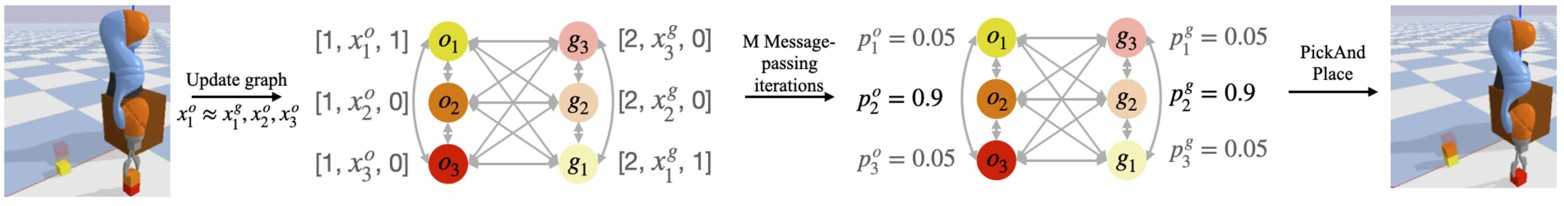
\includegraphics[width=1\textwidth]{figures/images/ch4/geometric_graph_computation.jpg}
    \caption{Computation flow in a scene represented by a Geometric Graph. Object nodes ($o_{i}$) and goal nodes ($g_{i}$) are created, with edges connecting them based on spatial and semantic relationships. A GNN classifies the nodes, selecting one object node and one goal node. These nodes are then passed as input to a motion primitive, which generates the necessary actions to move the selected object towards the target goal.}
    \label{fig:geometric_graph_computation}
\end{figure}

% \smalltodo{add figure}

A similar approach is presented in \cite{di2023one}, where two GNNs are trained separately to classify an object node and a goal node.

While these methods are noteworthy because they can solve multi-step tasks through supervised learning without relying on a planning algorithm, they have significant limitations. The most notable is their dependency on knowing both the current and target positions of the objects. In these early studies, such information is provided either by the simulation environment or by using special markers on objects in real-world settings to facilitate position estimation.

To address these limitations, the authors in \cite{zhu2021hierarchical} extended the Geometric Graph concept and proposed a new representation called the \textit{Symbolic Scene Graph}. In this framework, a 3D Object Pose Estimation module is used to extract objects from the scene, constructing a geometric graph. Edges are then added based on predefined relationships (e.g., ``can1 on shelf A", as illustrated in Figure \ref{fig:geometric_scene_graph}). The next step in the planning process is determined using a Neuro-Symbolic Task Planning module \cite{xu2019regression}, which takes the current Symbolic Scene Graph and the goal (expressed as desired predicates, i.e., relationships between objects) as input. This module outputs the next action, expressed as a subgoal achievable with a single motion primitive.
\begin{figure}[t]
    \centering
    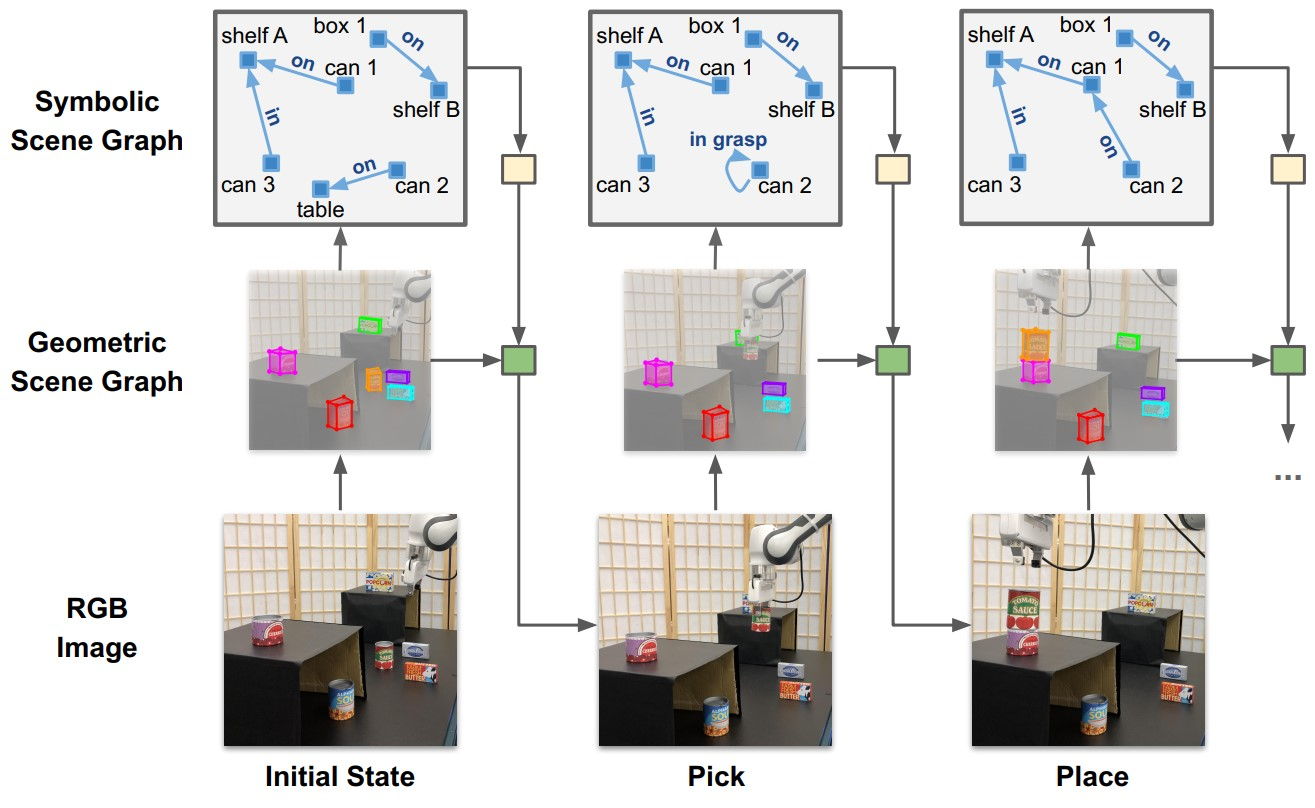
\includegraphics[width=0.8\textwidth]{figures/images/ch4/geometric_scene_graph.jpg}
    \caption{Example of a Symbolic Scene Graph. The graph is constructed by extracting objects from the scene and adding edges based on predefined relationships.}
    \label{fig:geometric_scene_graph}
\end{figure}


While this method showed promising results, including reduced computation times compared to the PDDLStream \cite{garrett2020pddlstream} baseline, it has limitations. The primary challenge lies in the cognitive module, which relies on 3D object pose estimation. This technique is only robust and reliable when used with pre-known objects.

\paragraph*{Conjugate Task Graph} \mbox{}\\
The Conjugate Task Graph (CTG) \cite{huang2019neural} addresses challenges in constructing traditional Task Graphs, where nodes represent states and edges represent transitions. For novel tasks, mapping states to new nodes is often infeasible. In contrast, the CTG uses nodes to represent actions, with edges implicitly representing states and their preconditions (Figure \ref{fig:conjugate_task_graph}).
\begin{figure}[t]
    \centering
    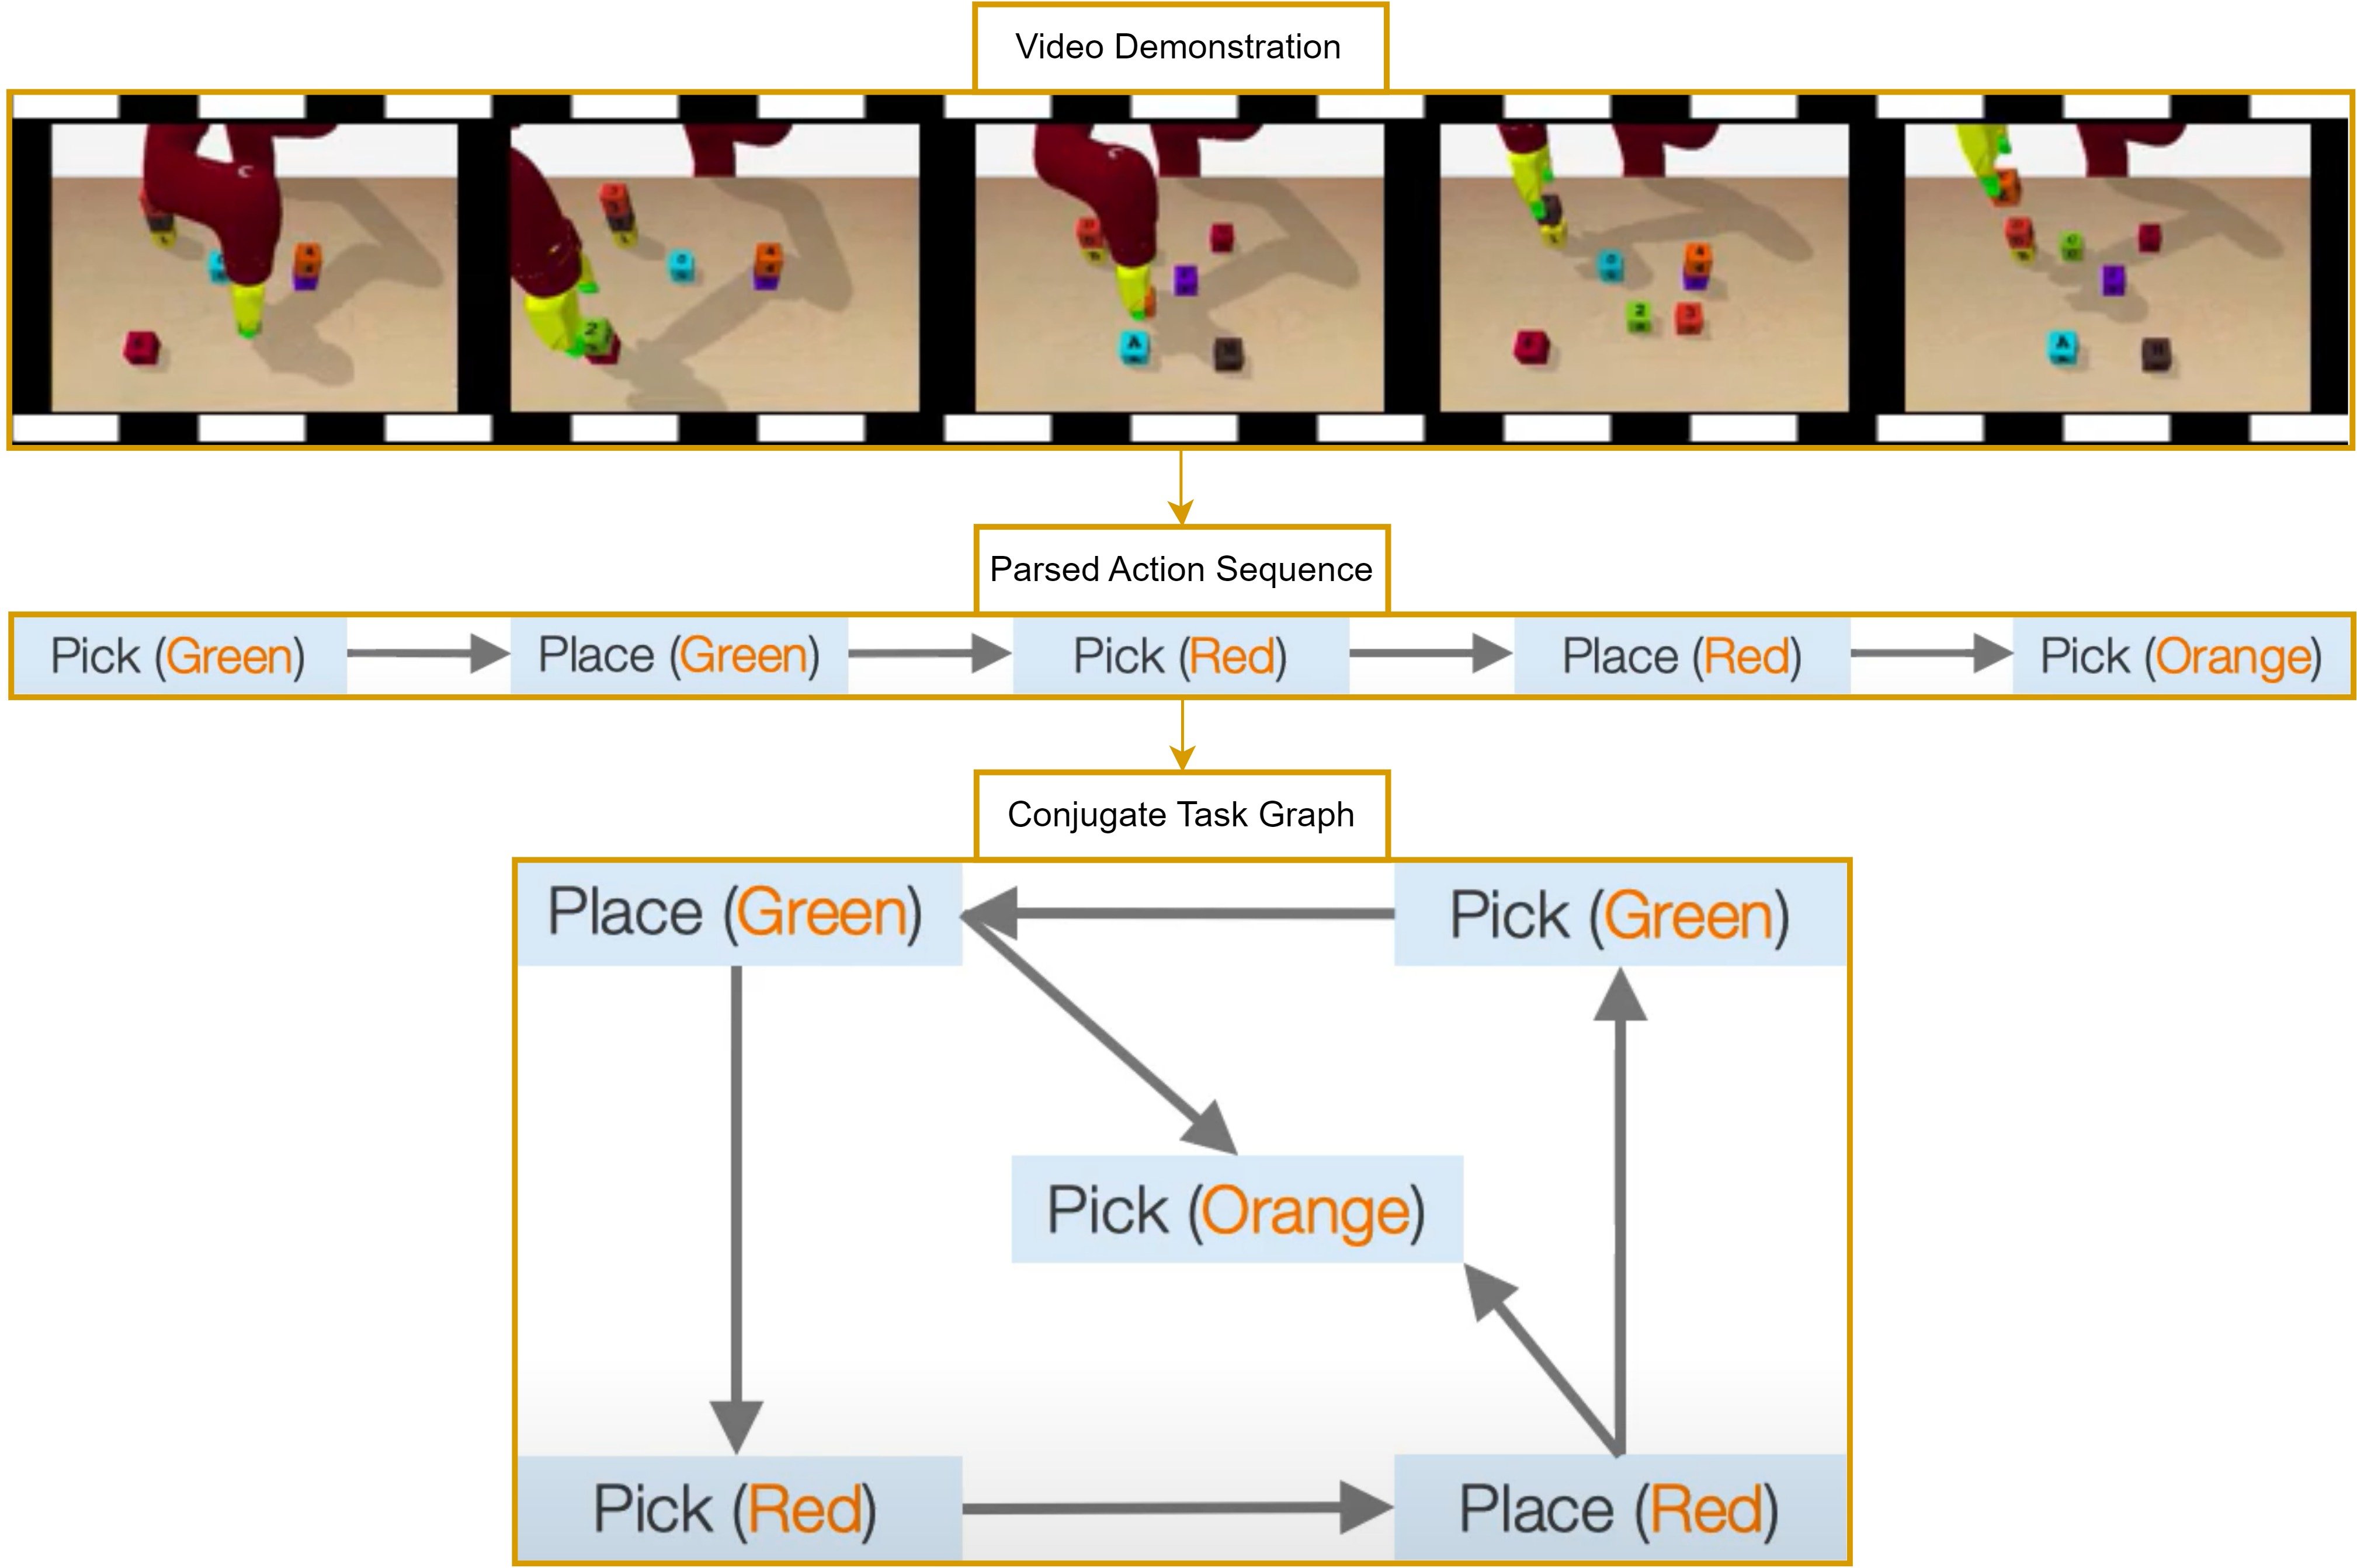
\includegraphics[width=0.8\textwidth]{figures/images/ch4/conjugate_task_graph.jpg}
    \caption{Conjugate Task Graph representation. Starting from the video demonstration, the sequence of actions is extracted and used to construct the initial graph. Then the complete Conjugate Task Graph is built by predicting the missing edges, which represents possible actions sequences observed in the training set.}
    \label{fig:conjugate_task_graph}
\end{figure}

Based on this representation, and assuming all possible actions have been observed in the training set, it is possible to build and train a modular architecture composed of the following components:
\begin{itemize}
    \item \textit{Demo Interpreter}: A Convolutional Neural Network \\ trained to extract the sequence of actions performed by a robot from a given demonstration. This sequence of actions is used to construct an initial graph.
    
    \item \textit{Graph Completion}: A Graph Neural Network trained to complete the graph produced by the Demo Interpreter. This module predicts the missing edges in the graph, representing unseen transitions between actions.
    
    \item \textit{Node Localization}: A Multi-Layer Perceptron that, given the current observation's encoding and the embeddings of the nodes in the graph, predicts the node corresponding to the action the robot is currently performing.
    
    \item \textit{Edge Localization}: Another MLP that, given the current observation's encoding and the node embeddings, predicts the edge representing the next transition and, consequently, the next action the robot should take.
\end{itemize}

The complete architecture was trained end-to-end, and experimental results demonstrate its effectiveness in multi-step tasks, such as object ordering and stacking. The CTG representation enables the policy to generalize to novel sequences of actions, making it particularly well-suited for tasks like object ordering.

However, this approach fails to generate valid paths when the demonstration includes out-of-distribution observations, produced by sequences of actions that were never encountered in the training set. Additionally, experimental results reveal that this method struggles to perform tasks requiring more than 6 steps. This limitation arises mainly from the Demo Interpreter module, which must generate long action sequences to instantiate the CTG.
